\documentclass[1p]{elsarticle_modified}
%\bibliographystyle{elsarticle-num}

%\usepackage[colorlinks]{hyperref}
%\usepackage{abbrmath_seonhwa} %\Abb, \Ascr, \Acal ,\Abf, \Afrak
\usepackage{amsfonts}
\usepackage{amssymb}
\usepackage{amsmath}
\usepackage{amsthm}
\usepackage{scalefnt}
\usepackage{amsbsy}
\usepackage{kotex}
\usepackage{caption}
\usepackage{subfig}
\usepackage{color}
\usepackage{graphicx}
\usepackage{xcolor} %% white, black, red, green, blue, cyan, magenta, yellow
\usepackage{float}
\usepackage{setspace}
\usepackage{hyperref}

\usepackage{tikz}
\usetikzlibrary{arrows}

\usepackage{multirow}
\usepackage{array} % fixed length table
\usepackage{hhline}

%%%%%%%%%%%%%%%%%%%%%
\makeatletter
\renewcommand*\env@matrix[1][\arraystretch]{%
	\edef\arraystretch{#1}%
	\hskip -\arraycolsep
	\let\@ifnextchar\new@ifnextchar
	\array{*\c@MaxMatrixCols c}}
\makeatother %https://tex.stackexchange.com/questions/14071/how-can-i-increase-the-line-spacing-in-a-matrix
%%%%%%%%%%%%%%%

\usepackage[normalem]{ulem}

\newcommand{\msout}[1]{\ifmmode\text{\sout{\ensuremath{#1}}}\else\sout{#1}\fi}
%SOURCE: \msout is \stkout macro in https://tex.stackexchange.com/questions/20609/strikeout-in-math-mode

\newcommand{\cancel}[1]{
	\ifmmode
	{\color{red}\msout{#1}}
	\else
	{\color{red}\sout{#1}}
	\fi
}

\newcommand{\add}[1]{
	{\color{blue}\uwave{#1}}
}

\newcommand{\replace}[2]{
	\ifmmode
	{\color{red}\msout{#1}}{\color{blue}\uwave{#2}}
	\else
	{\color{red}\sout{#1}}{\color{blue}\uwave{#2}}
	\fi
}

\newcommand{\Sol}{\mathcal{S}} %segment
\newcommand{\D}{D} %diagram
\newcommand{\A}{\mathcal{A}} %arc


%%%%%%%%%%%%%%%%%%%%%%%%%%%%%5 test

\def\sl{\operatorname{\textup{SL}}(2,\Cbb)}
\def\psl{\operatorname{\textup{PSL}}(2,\Cbb)}
\def\quan{\mkern 1mu \triangleright \mkern 1mu}

\theoremstyle{definition}
\newtheorem{thm}{Theorem}[section]
\newtheorem{prop}[thm]{Proposition}
\newtheorem{lem}[thm]{Lemma}
\newtheorem{ques}[thm]{Question}
\newtheorem{cor}[thm]{Corollary}
\newtheorem{defn}[thm]{Definition}
\newtheorem{exam}[thm]{Example}
\newtheorem{rmk}[thm]{Remark}
\newtheorem{alg}[thm]{Algorithm}

\newcommand{\I}{\sqrt{-1}}
\begin{document}

%\begin{frontmatter}
%
%\title{Boundary parabolic representations of knots up to 8 crossings}
%
%%% Group authors per affiliation:
%\author{Yunhi Cho} 
%\address{Department of Mathematics, University of Seoul, Seoul, Korea}
%\ead{yhcho@uos.ac.kr}
%
%
%\author{Seonhwa Kim} %\fnref{s_kim}}
%\address{Center for Geometry and Physics, Institute for Basic Science, Pohang, 37673, Korea}
%\ead{ryeona17@ibs.re.kr}
%
%\author{Hyuk Kim}
%\address{Department of Mathematical Sciences, Seoul National University, Seoul 08826, Korea}
%\ead{hyukkim@snu.ac.kr}
%
%\author{Seokbeom Yoon}
%\address{Department of Mathematical Sciences, Seoul National University, Seoul, 08826,  Korea}
%\ead{sbyoon15@snu.ac.kr}
%
%\begin{abstract}
%We find all boundary parabolic representation of knots up to 8 crossings.
%
%\end{abstract}
%\begin{keyword}
%    \MSC[2010] 57M25 
%\end{keyword}
%
%\end{frontmatter}

%\linenumbers
%\tableofcontents
%
\newcommand\colored[1]{\textcolor{white}{\rule[-0.35ex]{0.8em}{1.4ex}}\kern-0.8em\color{red} #1}%
%\newcommand\colored[1]{\textcolor{white}{ #1}\kern-2.17ex	\textcolor{white}{ #1}\kern-1.81ex	\textcolor{white}{ #1}\kern-2.15ex\color{red}#1	}

{\Large $\underline{12n_{0481}~(K12n_{0481})}$}

\setlength{\tabcolsep}{10pt}
\renewcommand{\arraystretch}{1.6}
\vspace{1cm}\begin{tabular}{m{100pt}>{\centering\arraybackslash}m{274pt}}
\multirow{5}{120pt}{
	\centering
	\includegraphics[width=112pt]{../../../GIT/diagram.site/Diagrams/png/2570_12n_0481.png}\\
\ \ \ A knot diagram\footnotemark}&
\allowdisplaybreaks
\textbf{Linearized knot diagam} \\
\cline{2-2}
 &
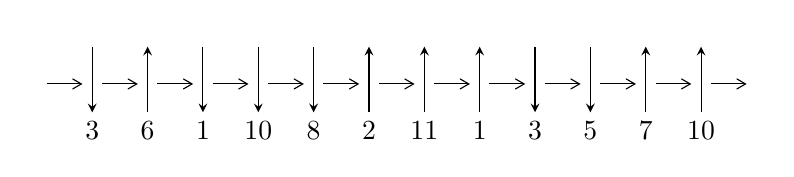
\begin{tikzpicture}[x=20pt, y=17pt]
	% nodes
	\node (C0) at (0, 0) {};
	\node (C1) at (1, 0) {};
	\node (C1U) at (1, +1) {};
	\node (C1D) at (1, -1) {3};

	\node (C2) at (2, 0) {};
	\node (C2U) at (2, +1) {};
	\node (C2D) at (2, -1) {6};

	\node (C3) at (3, 0) {};
	\node (C3U) at (3, +1) {};
	\node (C3D) at (3, -1) {1};

	\node (C4) at (4, 0) {};
	\node (C4U) at (4, +1) {};
	\node (C4D) at (4, -1) {10};

	\node (C5) at (5, 0) {};
	\node (C5U) at (5, +1) {};
	\node (C5D) at (5, -1) {8};

	\node (C6) at (6, 0) {};
	\node (C6U) at (6, +1) {};
	\node (C6D) at (6, -1) {2};

	\node (C7) at (7, 0) {};
	\node (C7U) at (7, +1) {};
	\node (C7D) at (7, -1) {11};

	\node (C8) at (8, 0) {};
	\node (C8U) at (8, +1) {};
	\node (C8D) at (8, -1) {1};

	\node (C9) at (9, 0) {};
	\node (C9U) at (9, +1) {};
	\node (C9D) at (9, -1) {3};

	\node (C10) at (10, 0) {};
	\node (C10U) at (10, +1) {};
	\node (C10D) at (10, -1) {5};

	\node (C11) at (11, 0) {};
	\node (C11U) at (11, +1) {};
	\node (C11D) at (11, -1) {7};

	\node (C12) at (12, 0) {};
	\node (C12U) at (12, +1) {};
	\node (C12D) at (12, -1) {10};
	\node (C13) at (13, 0) {};

	% arrows
	\draw[->,>={angle 60}]
	(C0) edge (C1) (C1) edge (C2) (C2) edge (C3) (C3) edge (C4) (C4) edge (C5) (C5) edge (C6) (C6) edge (C7) (C7) edge (C8) (C8) edge (C9) (C9) edge (C10) (C10) edge (C11) (C11) edge (C12) (C12) edge (C13) ;	\draw[->,>=stealth]
	(C1U) edge (C1D) (C2D) edge (C2U) (C3U) edge (C3D) (C4U) edge (C4D) (C5U) edge (C5D) (C6D) edge (C6U) (C7D) edge (C7U) (C8D) edge (C8U) (C9U) edge (C9D) (C10U) edge (C10D) (C11D) edge (C11U) (C12D) edge (C12U) ;
	\end{tikzpicture} \\
\hhline{~~} \\& 
\textbf{Solving Sequence} \\ \cline{2-2} 
 &
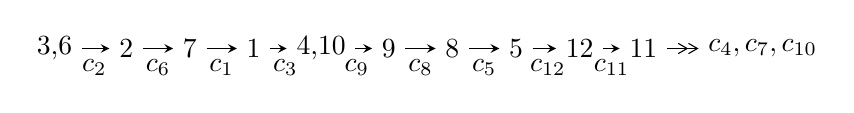
\begin{tikzpicture}[x=23pt, y=7pt]
	% node
	\node (A0) at (-1/8, 0) {3,6};
	\node (A1) at (1, 0) {2};
	\node (A2) at (2, 0) {7};
	\node (A3) at (3, 0) {1};
	\node (A4) at (65/16, 0) {4,10};
	\node (A5) at (41/8, 0) {9};
	\node (A6) at (49/8, 0) {8};
	\node (A7) at (57/8, 0) {5};
	\node (A8) at (65/8, 0) {12};
	\node (A9) at (73/8, 0) {11};
	\node (C1) at (1/2, -1) {$c_{2}$};
	\node (C2) at (3/2, -1) {$c_{6}$};
	\node (C3) at (5/2, -1) {$c_{1}$};
	\node (C4) at (7/2, -1) {$c_{3}$};
	\node (C5) at (37/8, -1) {$c_{9}$};
	\node (C6) at (45/8, -1) {$c_{8}$};
	\node (C7) at (53/8, -1) {$c_{5}$};
	\node (C8) at (61/8, -1) {$c_{12}$};
	\node (C9) at (69/8, -1) {$c_{11}$};
	\node (A10) at (11, 0) {$c_{4},c_{7},c_{10}$};

	% edge
	\draw[->,>=stealth]	
	(A0) edge (A1) (A1) edge (A2) (A2) edge (A3) (A3) edge (A4) (A4) edge (A5) (A5) edge (A6) (A6) edge (A7) (A7) edge (A8) (A8) edge (A9) ;
	\draw[->>,>={angle 60}]	
	(A9) edge (A10);
\end{tikzpicture} \\ 

\end{tabular} \\

\footnotetext{
The image of knot diagram is generated by the software ``\textbf{Draw programme}" developed by Andrew Bartholomew(\url{http://www.layer8.co.uk/maths/draw/index.htm\#Running-draw}), where we modified some parts for our purpose(\url{https://github.com/CATsTAILs/LinksPainter}).
}\phantom \\ \newline 
\centering \textbf{Ideals for irreducible components\footnotemark of $X_{\text{par}}$} 
 
\begin{align*}
I^u_{1}&=\langle 
u^{23}+2 u^{22}+\cdots+2 b+2,\;u^{23}+4 u^{22}+\cdots+4 a+12,\;u^{24}+6 u^{23}+\cdots+14 u+4\rangle \\
I^u_{2}&=\langle 
u^{14}- u^{13}+2 u^{12}-2 u^{11}+6 u^{10}-5 u^9+7 u^8-7 u^7+9 u^6-8 u^5+7 u^4-7 u^3+4 u^2+b-3 u+2,\\
\phantom{I^u_{2}}&\phantom{= \langle  }-2 u^{15}+2 u^{14}+\cdots+a-1,\\
\phantom{I^u_{2}}&\phantom{= \langle  }u^{16}- u^{15}+3 u^{14}-2 u^{13}+8 u^{12}-5 u^{11}+13 u^{10}-6 u^9+17 u^8-7 u^7+17 u^6-6 u^5+12 u^4-3 u^3+6 u^2- u+1\rangle \\
I^u_{3}&=\langle 
-59 u^5 a^3+81 u^5 a^2+\cdots-15 a+343,\;u^5 a^3+4 u^5 a^2+\cdots-4 a+8,\;u^6- u^5+u^4+2 u^2- u+1\rangle \\
\\
\end{align*}
\raggedright * 3 irreducible components of $\dim_{\mathbb{C}}=0$, with total 64 representations.\\
\footnotetext{All coefficients of polynomials are rational numbers. But the coefficients are sometimes approximated in decimal forms when there is not enough margin.}
\newpage
\renewcommand{\arraystretch}{1}
\centering \section*{I. $I^u_{1}= \langle u^{23}+2 u^{22}+\cdots+2 b+2,\;u^{23}+4 u^{22}+\cdots+4 a+12,\;u^{24}+6 u^{23}+\cdots+14 u+4 \rangle$}
\flushleft \textbf{(i) Arc colorings}\\
\begin{tabular}{m{7pt} m{180pt} m{7pt} m{180pt} }
\flushright $a_{3}=$&$\begin{pmatrix}1\\0\end{pmatrix}$ \\
\flushright $a_{6}=$&$\begin{pmatrix}0\\u\end{pmatrix}$ \\
\flushright $a_{2}=$&$\begin{pmatrix}1\\u^2\end{pmatrix}$ \\
\flushright $a_{7}=$&$\begin{pmatrix}u\\u^3+u\end{pmatrix}$ \\
\flushright $a_{1}=$&$\begin{pmatrix}u^2+1\\u^2\end{pmatrix}$ \\
\flushright $a_{4}=$&$\begin{pmatrix}u^4+u^2+1\\u^4\end{pmatrix}$ \\
\flushright $a_{10}=$&$\begin{pmatrix}-\frac{1}{4} u^{23}- u^{22}+\cdots-\frac{31}{4} u-3\\-\frac{1}{2} u^{23}- u^{22}+\cdots-\frac{1}{2} u-1\end{pmatrix}$ \\
\flushright $a_{9}=$&$\begin{pmatrix}-\frac{3}{4} u^{23}-2 u^{22}+\cdots-\frac{33}{4} u-4\\-\frac{1}{2} u^{23}- u^{22}+\cdots-\frac{1}{2} u-1\end{pmatrix}$ \\
\flushright $a_{8}=$&$\begin{pmatrix}\frac{3}{4} u^{23}- u^{22}+\cdots-\frac{87}{4} u-9\\\frac{5}{2} u^{23}+8 u^{22}+\cdots-\frac{17}{2} u-5\end{pmatrix}$ \\
\flushright $a_{5}=$&$\begin{pmatrix}-\frac{1}{2} u^{23}-\frac{5}{2} u^{22}+\cdots-\frac{7}{2} u-\frac{1}{2}\\-\frac{1}{2} u^{23}-3 u^{22}+\cdots-\frac{11}{2} u-2\end{pmatrix}$ \\
\flushright $a_{12}=$&$\begin{pmatrix}u^{23}-\frac{3}{2} u^{22}+\cdots-34 u-\frac{29}{2}\\\frac{15}{2} u^{23}+34 u^{22}+\cdots+\frac{59}{2} u+4\end{pmatrix}$ \\
\flushright $a_{11}=$&$\begin{pmatrix}-\frac{1}{2} u^{22}-2 u^{21}+\cdots-3 u-\frac{1}{2}\\-\frac{7}{2} u^{23}-19 u^{22}+\cdots-\frac{67}{2} u-10\end{pmatrix}$\\&\end{tabular}
\flushleft \textbf{(ii) Obstruction class $= -1$}\\~\\
\flushleft \textbf{(iii) Cusp Shapes $= 3 u^{23}+16 u^{22}+53 u^{21}+118 u^{20}+215 u^{19}+322 u^{18}+436 u^{17}+502 u^{16}+531 u^{15}+480 u^{14}+441 u^{13}+369 u^{12}+374 u^{11}+355 u^{10}+392 u^9+344 u^8+324 u^7+245 u^6+196 u^5+117 u^4+92 u^3+68 u^2+48 u+14$}\\~\\
\newpage\renewcommand{\arraystretch}{1}
\flushleft \textbf{(iv) u-Polynomials at the component}\newline \\
\begin{tabular}{m{50pt}|m{274pt}}
Crossings & \hspace{64pt}u-Polynomials at each crossing \\
\hline $$\begin{aligned}c_{1},c_{3}\end{aligned}$$&$\begin{aligned}
&u^{24}+6 u^{23}+\cdots+52 u+16
\end{aligned}$\\
\hline $$\begin{aligned}c_{2},c_{6}\end{aligned}$$&$\begin{aligned}
&u^{24}-6 u^{23}+\cdots-14 u+4
\end{aligned}$\\
\hline $$\begin{aligned}c_{4},c_{5},c_{10}\end{aligned}$$&$\begin{aligned}
&u^{24}- u^{23}+\cdots+2 u+1
\end{aligned}$\\
\hline $$\begin{aligned}c_{7},c_{11}\end{aligned}$$&$\begin{aligned}
&u^{24}-15 u^{23}+\cdots-544 u+64
\end{aligned}$\\
\hline $$\begin{aligned}c_{8}\end{aligned}$$&$\begin{aligned}
&u^{24}-2 u^{23}+\cdots-99 u+41
\end{aligned}$\\
\hline $$\begin{aligned}c_{9}\end{aligned}$$&$\begin{aligned}
&u^{24}+29 u^{22}+\cdots+4 u+1
\end{aligned}$\\
\hline $$\begin{aligned}c_{12}\end{aligned}$$&$\begin{aligned}
&u^{24}+3 u^{23}+\cdots+16 u+1
\end{aligned}$\\
\hline
\end{tabular}\\~\\
\newpage\renewcommand{\arraystretch}{1}
\flushleft \textbf{(v) Riley Polynomials at the component}\newline \\
\begin{tabular}{m{50pt}|m{274pt}}
Crossings & \hspace{64pt}Riley Polynomials at each crossing \\
\hline $$\begin{aligned}c_{1},c_{3}\end{aligned}$$&$\begin{aligned}
&y^{24}+26 y^{23}+\cdots+5520 y+256
\end{aligned}$\\
\hline $$\begin{aligned}c_{2},c_{6}\end{aligned}$$&$\begin{aligned}
&y^{24}+6 y^{23}+\cdots+52 y+16
\end{aligned}$\\
\hline $$\begin{aligned}c_{4},c_{5},c_{10}\end{aligned}$$&$\begin{aligned}
&y^{24}-11 y^{23}+\cdots-6 y+1
\end{aligned}$\\
\hline $$\begin{aligned}c_{7},c_{11}\end{aligned}$$&$\begin{aligned}
&y^{24}+7 y^{23}+\cdots+48128 y+4096
\end{aligned}$\\
\hline $$\begin{aligned}c_{8}\end{aligned}$$&$\begin{aligned}
&y^{24}-54 y^{23}+\cdots+14635 y+1681
\end{aligned}$\\
\hline $$\begin{aligned}c_{9}\end{aligned}$$&$\begin{aligned}
&y^{24}+58 y^{23}+\cdots+8 y+1
\end{aligned}$\\
\hline $$\begin{aligned}c_{12}\end{aligned}$$&$\begin{aligned}
&y^{24}-45 y^{23}+\cdots-10 y+1
\end{aligned}$\\
\hline
\end{tabular}\\~\\
\newpage\flushleft \textbf{(vi) Complex Volumes and Cusp Shapes}
$$\begin{array}{c|c|c}  
\text{Solutions to }I^u_{1}& \I (\text{vol} + \sqrt{-1}CS) & \text{Cusp shape}\\
 \hline 
\begin{aligned}
u &= \phantom{-}0.386803 + 0.939568 I \\
a &= \phantom{-}0.546906 + 0.473576 I \\
b &= \phantom{-}0.233412 - 0.697036 I\end{aligned}
 & \phantom{-}1.14776 + 2.44837 I & -4.92674 - 7.51322 I \\ \hline\begin{aligned}
u &= \phantom{-}0.386803 - 0.939568 I \\
a &= \phantom{-}0.546906 - 0.473576 I \\
b &= \phantom{-}0.233412 + 0.697036 I\end{aligned}
 & \phantom{-}1.14776 - 2.44837 I & -4.92674 + 7.51322 I \\ \hline\begin{aligned}
u &= \phantom{-}0.848616 + 0.384852 I \\
a &= \phantom{-}0.386852 - 0.278466 I \\
b &= -0.435457 + 0.087430 I\end{aligned}
 & -0.11794 - 4.13281 I & \phantom{-}1.46214 + 3.63821 I \\ \hline\begin{aligned}
u &= \phantom{-}0.848616 - 0.384852 I \\
a &= \phantom{-}0.386852 + 0.278466 I \\
b &= -0.435457 - 0.087430 I\end{aligned}
 & -0.11794 + 4.13281 I & \phantom{-}1.46214 - 3.63821 I \\ \hline\begin{aligned}
u &= \phantom{-}0.040508 + 1.108090 I \\
a &= -0.488177 + 0.024616 I \\
b &= \phantom{-}0.047052 + 0.539945 I\end{aligned}
 & -5.52346 - 2.09827 I & -4.00959 + 3.29797 I \\ \hline\begin{aligned}
u &= \phantom{-}0.040508 - 1.108090 I \\
a &= -0.488177 - 0.024616 I \\
b &= \phantom{-}0.047052 - 0.539945 I\end{aligned}
 & -5.52346 + 2.09827 I & -4.00959 - 3.29797 I \\ \hline\begin{aligned}
u &= -0.655613 + 0.578423 I \\
a &= \phantom{-}0.092968 - 0.792314 I \\
b &= -0.397342 - 0.573226 I\end{aligned}
 & -0.030667 - 0.985462 I & \phantom{-}0.04895 + 2.32635 I \\ \hline\begin{aligned}
u &= -0.655613 - 0.578423 I \\
a &= \phantom{-}0.092968 + 0.792314 I \\
b &= -0.397342 + 0.573226 I\end{aligned}
 & -0.030667 + 0.985462 I & \phantom{-}0.04895 - 2.32635 I \\ \hline\begin{aligned}
u &= \phantom{-}0.520277 + 1.085810 I \\
a &= -0.285416 - 0.342185 I \\
b &= -0.223052 + 0.487939 I\end{aligned}
 & -2.45634 + 9.15615 I & -2.49184 - 8.31719 I \\ \hline\begin{aligned}
u &= \phantom{-}0.520277 - 1.085810 I \\
a &= -0.285416 + 0.342185 I \\
b &= -0.223052 - 0.487939 I\end{aligned}
 & -2.45634 - 9.15615 I & -2.49184 + 8.31719 I\\
 \hline 
 \end{array}$$\newpage$$\begin{array}{c|c|c}  
\text{Solutions to }I^u_{1}& \I (\text{vol} + \sqrt{-1}CS) & \text{Cusp shape}\\
 \hline 
\begin{aligned}
u &= -0.658406 + 1.013050 I \\
a &= \phantom{-}0.733469 - 0.062319 I \\
b &= \phantom{-}0.419788 - 0.784073 I\end{aligned}
 & -1.23495 - 4.21264 I & -0.00163 + 4.38379 I \\ \hline\begin{aligned}
u &= -0.658406 - 1.013050 I \\
a &= \phantom{-}0.733469 + 0.062319 I \\
b &= \phantom{-}0.419788 + 0.784073 I\end{aligned}
 & -1.23495 + 4.21264 I & -0.00163 - 4.38379 I \\ \hline\begin{aligned}
u &= \phantom{-}0.581550 + 0.531676 I \\
a &= -0.473776 + 0.623048 I \\
b &= \phantom{-}0.606784 - 0.110438 I\end{aligned}
 & \phantom{-}2.58155 + 1.28427 I & \phantom{-}4.89493 + 0.75788 I \\ \hline\begin{aligned}
u &= \phantom{-}0.581550 - 0.531676 I \\
a &= -0.473776 - 0.623048 I \\
b &= \phantom{-}0.606784 + 0.110438 I\end{aligned}
 & \phantom{-}2.58155 - 1.28427 I & \phantom{-}4.89493 - 0.75788 I \\ \hline\begin{aligned}
u &= -0.932185 + 0.856145 I \\
a &= -0.97723 + 1.89200 I \\
b &= \phantom{-}0.70887 + 2.60034 I\end{aligned}
 & \phantom{-}10.05900 - 0.11341 I & \phantom{-}1.099246 + 0.004662 I \\ \hline\begin{aligned}
u &= -0.932185 - 0.856145 I \\
a &= -0.97723 - 1.89200 I \\
b &= \phantom{-}0.70887 - 2.60034 I\end{aligned}
 & \phantom{-}10.05900 + 0.11341 I & \phantom{-}1.099246 - 0.004662 I \\ \hline\begin{aligned}
u &= -0.973395 + 0.865459 I \\
a &= \phantom{-}1.26433 - 1.54946 I \\
b &= -0.11030 - 2.60246 I\end{aligned}
 & \phantom{-}8.07660 + 7.22190 I & \phantom{-}0.55503 - 3.04448 I \\ \hline\begin{aligned}
u &= -0.973395 - 0.865459 I \\
a &= \phantom{-}1.26433 + 1.54946 I \\
b &= -0.11030 + 2.60246 I\end{aligned}
 & \phantom{-}8.07660 - 7.22190 I & \phantom{-}0.55503 + 3.04448 I \\ \hline\begin{aligned}
u &= -0.858450 + 1.000080 I \\
a &= -1.68242 + 1.24146 I \\
b &= -0.20271 + 2.74829 I\end{aligned}
 & \phantom{-}9.58925 - 6.48997 I & \phantom{-}0.12796 + 4.63982 I \\ \hline\begin{aligned}
u &= -0.858450 - 1.000080 I \\
a &= -1.68242 - 1.24146 I \\
b &= -0.20271 - 2.74829 I\end{aligned}
 & \phantom{-}9.58925 + 6.48997 I & \phantom{-}0.12796 - 4.63982 I\\
 \hline 
 \end{array}$$\newpage$$\begin{array}{c|c|c}  
\text{Solutions to }I^u_{1}& \I (\text{vol} + \sqrt{-1}CS) & \text{Cusp shape}\\
 \hline 
\begin{aligned}
u &= -0.886343 + 1.020850 I \\
a &= \phantom{-}1.33428 - 1.55406 I \\
b &= -0.40384 - 2.73953 I\end{aligned}
 & \phantom{-}7.5650 - 14.0430 I & -0.21532 + 7.35996 I \\ \hline\begin{aligned}
u &= -0.886343 - 1.020850 I \\
a &= \phantom{-}1.33428 + 1.55406 I \\
b &= -0.40384 + 2.73953 I\end{aligned}
 & \phantom{-}7.5650 + 14.0430 I & -0.21532 - 7.35996 I \\ \hline\begin{aligned}
u &= -0.413363 + 0.497922 I \\
a &= \phantom{-}0.298212 - 0.736016 I \\
b &= -0.243208 - 0.452728 I\end{aligned}
 & -0.046922 - 1.057330 I & -0.54314 + 5.53414 I \\ \hline\begin{aligned}
u &= -0.413363 - 0.497922 I \\
a &= \phantom{-}0.298212 + 0.736016 I \\
b &= -0.243208 + 0.452728 I\end{aligned}
 & -0.046922 + 1.057330 I & -0.54314 - 5.53414 I\\
 \hline 
 \end{array}$$\newpage\newpage\renewcommand{\arraystretch}{1}
\centering \section*{II. $I^u_{2}= \langle u^{14}- u^{13}+\cdots+b+2,\;-2 u^{15}+2 u^{14}+\cdots+a-1,\;u^{16}- u^{15}+\cdots- u+1 \rangle$}
\flushleft \textbf{(i) Arc colorings}\\
\begin{tabular}{m{7pt} m{180pt} m{7pt} m{180pt} }
\flushright $a_{3}=$&$\begin{pmatrix}1\\0\end{pmatrix}$ \\
\flushright $a_{6}=$&$\begin{pmatrix}0\\u\end{pmatrix}$ \\
\flushright $a_{2}=$&$\begin{pmatrix}1\\u^2\end{pmatrix}$ \\
\flushright $a_{7}=$&$\begin{pmatrix}u\\u^3+u\end{pmatrix}$ \\
\flushright $a_{1}=$&$\begin{pmatrix}u^2+1\\u^2\end{pmatrix}$ \\
\flushright $a_{4}=$&$\begin{pmatrix}u^4+u^2+1\\u^4\end{pmatrix}$ \\
\flushright $a_{10}=$&$\begin{pmatrix}2 u^{15}-2 u^{14}+\cdots+8 u+1\\- u^{14}+u^{13}+\cdots+3 u-2\end{pmatrix}$ \\
\flushright $a_{9}=$&$\begin{pmatrix}2 u^{15}-3 u^{14}+\cdots+11 u-1\\- u^{14}+u^{13}+\cdots+3 u-2\end{pmatrix}$ \\
\flushright $a_{8}=$&$\begin{pmatrix}2 u^{15}-2 u^{14}+\cdots- u^2+8 u\\u^{15}-2 u^{14}+\cdots+5 u-3\end{pmatrix}$ \\
\flushright $a_{5}=$&$\begin{pmatrix}-2 u^{15}+u^{14}+\cdots-9 u-2\\- u^{15}+u^{14}+\cdots-5 u+2\end{pmatrix}$ \\
\flushright $a_{12}=$&$\begin{pmatrix}- u^{14}+u^{13}+\cdots- u-4\\- u^{15}+u^{14}+\cdots-11 u^3-5 u\end{pmatrix}$ \\
\flushright $a_{11}=$&$\begin{pmatrix}- u^{15}-2 u^{13}+\cdots-3 u-3\\-2 u^{15}+2 u^{14}+\cdots-6 u+1\end{pmatrix}$\\&\end{tabular}
\flushleft \textbf{(ii) Obstruction class $= 1$}\\~\\
\flushleft \textbf{(iii) Cusp Shapes $= -2 u^{14}+u^{13}-7 u^{12}+2 u^{11}-15 u^{10}+3 u^9-28 u^8+3 u^7-29 u^6+2 u^5-32 u^4+3 u^3-18 u^2+u-10$}\\~\\
\newpage\renewcommand{\arraystretch}{1}
\flushleft \textbf{(iv) u-Polynomials at the component}\newline \\
\begin{tabular}{m{50pt}|m{274pt}}
Crossings & \hspace{64pt}u-Polynomials at each crossing \\
\hline $$\begin{aligned}c_{1}\end{aligned}$$&$\begin{aligned}
&u^{16}-5 u^{15}+\cdots-11 u+1
\end{aligned}$\\
\hline $$\begin{aligned}c_{2}\end{aligned}$$&$\begin{aligned}
&u^{16}- u^{15}+\cdots- u+1
\end{aligned}$\\
\hline $$\begin{aligned}c_{3}\end{aligned}$$&$\begin{aligned}
&u^{16}+5 u^{15}+\cdots+11 u+1
\end{aligned}$\\
\hline $$\begin{aligned}c_{4}\end{aligned}$$&$\begin{aligned}
&u^{16}+u^{15}+\cdots+4 u+1
\end{aligned}$\\
\hline $$\begin{aligned}c_{5},c_{10}\end{aligned}$$&$\begin{aligned}
&u^{16}- u^{15}+\cdots-4 u+1
\end{aligned}$\\
\hline $$\begin{aligned}c_{6}\end{aligned}$$&$\begin{aligned}
&u^{16}+u^{15}+\cdots+u+1
\end{aligned}$\\
\hline $$\begin{aligned}c_{7}\end{aligned}$$&$\begin{aligned}
&u^{16}-2 u^{15}+\cdots+3 u+1
\end{aligned}$\\
\hline $$\begin{aligned}c_{8}\end{aligned}$$&$\begin{aligned}
&u^{16}-2 u^{15}+\cdots+63 u+47
\end{aligned}$\\
\hline $$\begin{aligned}c_{9}\end{aligned}$$&$\begin{aligned}
&u^{16}-2 u^{14}+\cdots+2 u+1
\end{aligned}$\\
\hline $$\begin{aligned}c_{11}\end{aligned}$$&$\begin{aligned}
&u^{16}+2 u^{15}+\cdots-3 u+1
\end{aligned}$\\
\hline $$\begin{aligned}c_{12}\end{aligned}$$&$\begin{aligned}
&u^{16}-3 u^{15}+\cdots+2 u+1
\end{aligned}$\\
\hline
\end{tabular}\\~\\
\newpage\renewcommand{\arraystretch}{1}
\flushleft \textbf{(v) Riley Polynomials at the component}\newline \\
\begin{tabular}{m{50pt}|m{274pt}}
Crossings & \hspace{64pt}Riley Polynomials at each crossing \\
\hline $$\begin{aligned}c_{1},c_{3}\end{aligned}$$&$\begin{aligned}
&y^{16}+17 y^{15}+\cdots-13 y+1
\end{aligned}$\\
\hline $$\begin{aligned}c_{2},c_{6}\end{aligned}$$&$\begin{aligned}
&y^{16}+5 y^{15}+\cdots+11 y+1
\end{aligned}$\\
\hline $$\begin{aligned}c_{4},c_{5},c_{10}\end{aligned}$$&$\begin{aligned}
&y^{16}-13 y^{15}+\cdots+2 y+1
\end{aligned}$\\
\hline $$\begin{aligned}c_{7},c_{11}\end{aligned}$$&$\begin{aligned}
&y^{16}+6 y^{15}+\cdots-3 y+1
\end{aligned}$\\
\hline $$\begin{aligned}c_{8}\end{aligned}$$&$\begin{aligned}
&y^{16}-14 y^{14}+\cdots+10319 y+2209
\end{aligned}$\\
\hline $$\begin{aligned}c_{9}\end{aligned}$$&$\begin{aligned}
&y^{16}-4 y^{15}+\cdots-8 y+1
\end{aligned}$\\
\hline $$\begin{aligned}c_{12}\end{aligned}$$&$\begin{aligned}
&y^{16}-3 y^{15}+\cdots+6 y+1
\end{aligned}$\\
\hline
\end{tabular}\\~\\
\newpage\flushleft \textbf{(vi) Complex Volumes and Cusp Shapes}
$$\begin{array}{c|c|c}  
\text{Solutions to }I^u_{2}& \I (\text{vol} + \sqrt{-1}CS) & \text{Cusp shape}\\
 \hline 
\begin{aligned}
u &= \phantom{-}0.711929 + 0.760358 I \\
a &= -1.02576 + 1.48549 I \\
b &= -1.85977 + 0.27762 I\end{aligned}
 & -2.76244 - 0.95558 I & -1.206885 + 0.230523 I \\ \hline\begin{aligned}
u &= \phantom{-}0.711929 - 0.760358 I \\
a &= -1.02576 - 1.48549 I \\
b &= -1.85977 - 0.27762 I\end{aligned}
 & -2.76244 + 0.95558 I & -1.206885 - 0.230523 I \\ \hline\begin{aligned}
u &= \phantom{-}0.053541 + 0.950247 I \\
a &= -0.292929 - 0.930103 I \\
b &= \phantom{-}0.868144 - 0.328154 I\end{aligned}
 & -7.15170 - 1.53675 I & -10.75515 + 0.98813 I \\ \hline\begin{aligned}
u &= \phantom{-}0.053541 - 0.950247 I \\
a &= -0.292929 + 0.930103 I \\
b &= \phantom{-}0.868144 + 0.328154 I\end{aligned}
 & -7.15170 + 1.53675 I & -10.75515 - 0.98813 I \\ \hline\begin{aligned}
u &= -0.435996 + 0.803743 I \\
a &= \phantom{-}0.254017 - 0.569932 I \\
b &= \phantom{-}0.347329 + 0.452652 I\end{aligned}
 & \phantom{-}1.53953 - 1.76071 I & \phantom{-}0.705761 + 0.775767 I \\ \hline\begin{aligned}
u &= -0.435996 - 0.803743 I \\
a &= \phantom{-}0.254017 + 0.569932 I \\
b &= \phantom{-}0.347329 - 0.452652 I\end{aligned}
 & \phantom{-}1.53953 + 1.76071 I & \phantom{-}0.705761 - 0.775767 I \\ \hline\begin{aligned}
u &= -0.825406 + 0.738696 I \\
a &= -0.382034 - 0.004020 I \\
b &= \phantom{-}0.318303 - 0.278889 I\end{aligned}
 & -1.33661 - 2.36299 I & -2.87352 + 3.64592 I \\ \hline\begin{aligned}
u &= -0.825406 - 0.738696 I \\
a &= -0.382034 + 0.004020 I \\
b &= \phantom{-}0.318303 + 0.278889 I\end{aligned}
 & -1.33661 + 2.36299 I & -2.87352 - 3.64592 I \\ \hline\begin{aligned}
u &= \phantom{-}0.682235 + 0.952556 I \\
a &= \phantom{-}1.22003 - 0.92717 I \\
b &= \phantom{-}1.71553 + 0.52960 I\end{aligned}
 & -3.35855 + 6.31371 I & -2.68318 - 5.80907 I \\ \hline\begin{aligned}
u &= \phantom{-}0.682235 - 0.952556 I \\
a &= \phantom{-}1.22003 + 0.92717 I \\
b &= \phantom{-}1.71553 - 0.52960 I\end{aligned}
 & -3.35855 - 6.31371 I & -2.68318 + 5.80907 I\\
 \hline 
 \end{array}$$\newpage$$\begin{array}{c|c|c}  
\text{Solutions to }I^u_{2}& \I (\text{vol} + \sqrt{-1}CS) & \text{Cusp shape}\\
 \hline 
\begin{aligned}
u &= -0.724914 + 1.000500 I \\
a &= \phantom{-}0.270608 + 0.089531 I \\
b &= -0.285742 + 0.205840 I\end{aligned}
 & -2.17699 - 3.46039 I & -4.93993 + 0.90325 I \\ \hline\begin{aligned}
u &= -0.724914 - 1.000500 I \\
a &= \phantom{-}0.270608 - 0.089531 I \\
b &= -0.285742 - 0.205840 I\end{aligned}
 & -2.17699 + 3.46039 I & -4.93993 - 0.90325 I \\ \hline\begin{aligned}
u &= \phantom{-}0.922397 + 0.947682 I \\
a &= -1.20870 - 1.44097 I \\
b &= \phantom{-}0.25067 - 2.47461 I\end{aligned}
 & \phantom{-}10.66490 + 3.39525 I & \phantom{-}0.77812 - 2.38843 I \\ \hline\begin{aligned}
u &= \phantom{-}0.922397 - 0.947682 I \\
a &= -1.20870 + 1.44097 I \\
b &= \phantom{-}0.25067 + 2.47461 I\end{aligned}
 & \phantom{-}10.66490 - 3.39525 I & \phantom{-}0.77812 + 2.38843 I \\ \hline\begin{aligned}
u &= \phantom{-}0.116214 + 0.507066 I \\
a &= \phantom{-}0.66477 + 2.82354 I \\
b &= -1.35447 + 0.66522 I\end{aligned}
 & -5.28775 + 2.24439 I & -7.02522 - 0.50668 I \\ \hline\begin{aligned}
u &= \phantom{-}0.116214 - 0.507066 I \\
a &= \phantom{-}0.66477 - 2.82354 I \\
b &= -1.35447 - 0.66522 I\end{aligned}
 & -5.28775 - 2.24439 I & -7.02522 + 0.50668 I\\
 \hline 
 \end{array}$$\newpage\newpage\renewcommand{\arraystretch}{1}
\centering \section*{III. $I^u_{3}= \langle -59 u^5 a^3+81 u^5 a^2+\cdots-15 a+343,\;u^5 a^3+4 u^5 a^2+\cdots-4 a+8,\;u^6- u^5+u^4+2 u^2- u+1 \rangle$}
\flushleft \textbf{(i) Arc colorings}\\
\begin{tabular}{m{7pt} m{180pt} m{7pt} m{180pt} }
\flushright $a_{3}=$&$\begin{pmatrix}1\\0\end{pmatrix}$ \\
\flushright $a_{6}=$&$\begin{pmatrix}0\\u\end{pmatrix}$ \\
\flushright $a_{2}=$&$\begin{pmatrix}1\\u^2\end{pmatrix}$ \\
\flushright $a_{7}=$&$\begin{pmatrix}u\\u^3+u\end{pmatrix}$ \\
\flushright $a_{1}=$&$\begin{pmatrix}u^2+1\\u^2\end{pmatrix}$ \\
\flushright $a_{4}=$&$\begin{pmatrix}u^4+u^2+1\\u^4\end{pmatrix}$ \\
\flushright $a_{10}=$&$\begin{pmatrix}a\\0.337143 a^{3} u^{5}-0.462857 a^{2} u^{5}+\cdots+0.0857143 a-1.96000\end{pmatrix}$ \\
\flushright $a_{9}=$&$\begin{pmatrix}0.337143 a^{3} u^{5}-0.462857 a^{2} u^{5}+\cdots+1.08571 a-1.96000\\0.337143 a^{3} u^{5}-0.462857 a^{2} u^{5}+\cdots+0.0857143 a-1.96000\end{pmatrix}$ \\
\flushright $a_{8}=$&$\begin{pmatrix}-0.177143 a^{3} u^{5}+0.0228571 a^{2} u^{5}+\cdots+0.514286 a-1.36000\\0.160000 a^{3} u^{5}-0.440000 a^{2} u^{5}+\cdots-0.400000 a-3.32000\end{pmatrix}$ \\
\flushright $a_{5}=$&$\begin{pmatrix}0.0971429 a^{3} u^{5}+0.697143 a^{2} u^{5}+\cdots+0.685714 a+1.52000\\\frac{3}{35} u^5 a^3+\frac{3}{35} u^5 a^2+\cdots+\frac{3}{7} a+\frac{12}{5}\end{pmatrix}$ \\
\flushright $a_{12}=$&$\begin{pmatrix}-0.0285714 a^{3} u^{5}-0.0285714 a^{2} u^{5}+\cdots+0.857143 a+3.20000\\0.0685714 a^{3} u^{5}+0.668571 a^{2} u^{5}+\cdots+1.54286 a+2.72000\end{pmatrix}$ \\
\flushright $a_{11}=$&$\begin{pmatrix}-0.0742857 a^{3} u^{5}-0.474286 a^{2} u^{5}+\cdots+0.828571 a+2.72000\\-0.102857 a^{3} u^{5}-0.502857 a^{2} u^{5}+\cdots+1.68571 a+1.92000\end{pmatrix}$\\&\end{tabular}
\flushleft \textbf{(ii) Obstruction class $= -1$}\\~\\
\flushleft \textbf{(iii) Cusp Shapes $= -\frac{144}{175} u^5 a^3-\frac{4}{175} u^5 a^2+\cdots+\frac{52}{35} a-\frac{66}{25}$}\\~\\
\newpage\renewcommand{\arraystretch}{1}
\flushleft \textbf{(iv) u-Polynomials at the component}\newline \\
\begin{tabular}{m{50pt}|m{274pt}}
Crossings & \hspace{64pt}u-Polynomials at each crossing \\
\hline $$\begin{aligned}c_{1},c_{3}\end{aligned}$$&$\begin{aligned}
&(u^6+u^5+5 u^4+4 u^3+6 u^2+3 u+1)^4
\end{aligned}$\\
\hline $$\begin{aligned}c_{2},c_{6}\end{aligned}$$&$\begin{aligned}
&(u^6+u^5+u^4+2 u^2+u+1)^4
\end{aligned}$\\
\hline $$\begin{aligned}c_{4},c_{5},c_{10}\end{aligned}$$&$\begin{aligned}
&u^{24}+u^{23}+\cdots-60 u+49
\end{aligned}$\\
\hline $$\begin{aligned}c_{7},c_{11}\end{aligned}$$&$\begin{aligned}
&(u^2+u+1)^{12}
\end{aligned}$\\
\hline $$\begin{aligned}c_{8}\end{aligned}$$&$\begin{aligned}
&u^{24}- u^{23}+\cdots-13006 u+1333
\end{aligned}$\\
\hline $$\begin{aligned}c_{9}\end{aligned}$$&$\begin{aligned}
&u^{24}+u^{23}+\cdots-31002 u+7693
\end{aligned}$\\
\hline $$\begin{aligned}c_{12}\end{aligned}$$&$\begin{aligned}
&u^{24}+3 u^{23}+\cdots+1484 u+193
\end{aligned}$\\
\hline
\end{tabular}\\~\\
\newpage\renewcommand{\arraystretch}{1}
\flushleft \textbf{(v) Riley Polynomials at the component}\newline \\
\begin{tabular}{m{50pt}|m{274pt}}
Crossings & \hspace{64pt}Riley Polynomials at each crossing \\
\hline $$\begin{aligned}c_{1},c_{3}\end{aligned}$$&$\begin{aligned}
&(y^6+9 y^5+29 y^4+40 y^3+22 y^2+3 y+1)^4
\end{aligned}$\\
\hline $$\begin{aligned}c_{2},c_{6}\end{aligned}$$&$\begin{aligned}
&(y^6+y^5+5 y^4+4 y^3+6 y^2+3 y+1)^4
\end{aligned}$\\
\hline $$\begin{aligned}c_{4},c_{5},c_{10}\end{aligned}$$&$\begin{aligned}
&y^{24}-9 y^{23}+\cdots+6984 y+2401
\end{aligned}$\\
\hline $$\begin{aligned}c_{7},c_{11}\end{aligned}$$&$\begin{aligned}
&(y^2+y+1)^{12}
\end{aligned}$\\
\hline $$\begin{aligned}c_{8}\end{aligned}$$&$\begin{aligned}
&y^{24}-29 y^{23}+\cdots-9462636 y+1776889
\end{aligned}$\\
\hline $$\begin{aligned}c_{9}\end{aligned}$$&$\begin{aligned}
&y^{24}+31 y^{23}+\cdots-496651436 y+59182249
\end{aligned}$\\
\hline $$\begin{aligned}c_{12}\end{aligned}$$&$\begin{aligned}
&y^{24}-21 y^{23}+\cdots+485848 y+37249
\end{aligned}$\\
\hline
\end{tabular}\\~\\
\newpage\flushleft \textbf{(vi) Complex Volumes and Cusp Shapes}
$$\begin{array}{c|c|c}  
\text{Solutions to }I^u_{3}& \I (\text{vol} + \sqrt{-1}CS) & \text{Cusp shape}\\
 \hline 
\begin{aligned}
u &= -0.716019 + 0.809696 I \\
a &= \phantom{-}0.176965 - 0.992700 I \\
b &= -0.974499 - 0.266636 I\end{aligned}
 & -0.291980 - 0.626084 I & -0.418854 - 0.066014 I \\ \hline\begin{aligned}
u &= -0.716019 + 0.809696 I \\
a &= -0.412453 - 0.838801 I \\
b &= -0.677074 - 0.854080 I\end{aligned}
 & -0.291980 - 0.626084 I & -0.418854 - 0.066014 I \\ \hline\begin{aligned}
u &= -0.716019 + 0.809696 I \\
a &= \phantom{-}1.168780 + 0.614777 I \\
b &= \phantom{-}0.461703 - 0.363781 I\end{aligned}
 & -0.29198 - 4.68585 I & -0.41885 + 6.86219 I \\ \hline\begin{aligned}
u &= -0.716019 + 0.809696 I \\
a &= \phantom{-}0.535089 + 0.097035 I \\
b &= \phantom{-}1.33465 - 0.50617 I\end{aligned}
 & -0.29198 - 4.68585 I & -0.41885 + 6.86219 I \\ \hline\begin{aligned}
u &= -0.716019 - 0.809696 I \\
a &= \phantom{-}0.176965 + 0.992700 I \\
b &= -0.974499 + 0.266636 I\end{aligned}
 & -0.291980 + 0.626084 I & -0.418854 + 0.066014 I \\ \hline\begin{aligned}
u &= -0.716019 - 0.809696 I \\
a &= -0.412453 + 0.838801 I \\
b &= -0.677074 + 0.854080 I\end{aligned}
 & -0.291980 + 0.626084 I & -0.418854 + 0.066014 I \\ \hline\begin{aligned}
u &= -0.716019 - 0.809696 I \\
a &= \phantom{-}1.168780 - 0.614777 I \\
b &= \phantom{-}0.461703 + 0.363781 I\end{aligned}
 & -0.29198 + 4.68585 I & -0.41885 - 6.86219 I \\ \hline\begin{aligned}
u &= -0.716019 - 0.809696 I \\
a &= \phantom{-}0.535089 - 0.097035 I \\
b &= \phantom{-}1.33465 + 0.50617 I\end{aligned}
 & -0.29198 + 4.68585 I & -0.41885 - 6.86219 I \\ \hline\begin{aligned}
u &= \phantom{-}0.283231 + 0.633899 I \\
a &= -0.168030 + 0.836853 I \\
b &= -2.00423 - 0.05495 I\end{aligned}
 & -5.19289 - 0.92118 I & -5.53615 - 2.71707 I \\ \hline\begin{aligned}
u &= \phantom{-}0.283231 + 0.633899 I \\
a &= -0.78124 + 1.88064 I \\
b &= -0.86094 + 1.36524 I\end{aligned}
 & -5.19289 + 3.13859 I & -5.53615 - 9.64527 I\\
 \hline 
 \end{array}$$\newpage$$\begin{array}{c|c|c}  
\text{Solutions to }I^u_{3}& \I (\text{vol} + \sqrt{-1}CS) & \text{Cusp shape}\\
 \hline 
\begin{aligned}
u &= \phantom{-}0.283231 + 0.633899 I \\
a &= -1.28946 - 1.93430 I \\
b &= \phantom{-}1.413410 - 0.037425 I\end{aligned}
 & -5.19289 + 3.13859 I & -5.53615 - 9.64527 I \\ \hline\begin{aligned}
u &= \phantom{-}0.283231 + 0.633899 I \\
a &= \phantom{-}1.24986 - 2.60330 I \\
b &= \phantom{-}0.578072 - 0.130508 I\end{aligned}
 & -5.19289 - 0.92118 I & -5.53615 - 2.71707 I \\ \hline\begin{aligned}
u &= \phantom{-}0.283231 - 0.633899 I \\
a &= -0.168030 - 0.836853 I \\
b &= -2.00423 + 0.05495 I\end{aligned}
 & -5.19289 + 0.92118 I & -5.53615 + 2.71707 I \\ \hline\begin{aligned}
u &= \phantom{-}0.283231 - 0.633899 I \\
a &= -0.78124 - 1.88064 I \\
b &= -0.86094 - 1.36524 I\end{aligned}
 & -5.19289 - 3.13859 I & -5.53615 + 9.64527 I \\ \hline\begin{aligned}
u &= \phantom{-}0.283231 - 0.633899 I \\
a &= -1.28946 + 1.93430 I \\
b &= \phantom{-}1.413410 + 0.037425 I\end{aligned}
 & -5.19289 - 3.13859 I & -5.53615 + 9.64527 I \\ \hline\begin{aligned}
u &= \phantom{-}0.283231 - 0.633899 I \\
a &= \phantom{-}1.24986 + 2.60330 I \\
b &= \phantom{-}0.578072 + 0.130508 I\end{aligned}
 & -5.19289 + 0.92118 I & -5.53615 + 2.71707 I \\ \hline\begin{aligned}
u &= \phantom{-}0.932789 + 0.951611 I \\
a &= -0.96648 - 1.44906 I \\
b &= \phantom{-}0.36444 - 2.60092 I\end{aligned}
 & \phantom{-}10.41970 + 5.45709 I & -0.04500 - 5.71634 I \\ \hline\begin{aligned}
u &= \phantom{-}0.932789 + 0.951611 I \\
a &= \phantom{-}1.13707 + 1.36590 I \\
b &= \phantom{-}0.10273 + 2.42307 I\end{aligned}
 & \phantom{-}10.41970 + 1.39732 I & -0.044996 + 1.211865 I \\ \hline\begin{aligned}
u &= \phantom{-}0.932789 + 0.951611 I \\
a &= -1.35254 - 1.21783 I \\
b &= \phantom{-}0.23916 - 2.35614 I\end{aligned}
 & \phantom{-}10.41970 + 1.39732 I & -0.044996 + 1.211865 I \\ \hline\begin{aligned}
u &= \phantom{-}0.932789 + 0.951611 I \\
a &= \phantom{-}1.20244 + 1.56163 I \\
b &= -0.47742 + 2.27137 I\end{aligned}
 & \phantom{-}10.41970 + 5.45709 I & -0.04500 - 5.71634 I\\
 \hline 
 \end{array}$$\newpage$$\begin{array}{c|c|c}  
\text{Solutions to }I^u_{3}& \I (\text{vol} + \sqrt{-1}CS) & \text{Cusp shape}\\
 \hline 
\begin{aligned}
u &= \phantom{-}0.932789 - 0.951611 I \\
a &= -0.96648 + 1.44906 I \\
b &= \phantom{-}0.36444 + 2.60092 I\end{aligned}
 & \phantom{-}10.41970 - 5.45709 I & -0.04500 + 5.71634 I \\ \hline\begin{aligned}
u &= \phantom{-}0.932789 - 0.951611 I \\
a &= \phantom{-}1.13707 - 1.36590 I \\
b &= \phantom{-}0.10273 - 2.42307 I\end{aligned}
 & \phantom{-}10.41970 - 1.39732 I & -0.044996 - 1.211865 I \\ \hline\begin{aligned}
u &= \phantom{-}0.932789 - 0.951611 I \\
a &= -1.35254 + 1.21783 I \\
b &= \phantom{-}0.23916 + 2.35614 I\end{aligned}
 & \phantom{-}10.41970 - 1.39732 I & -0.044996 - 1.211865 I \\ \hline\begin{aligned}
u &= \phantom{-}0.932789 - 0.951611 I \\
a &= \phantom{-}1.20244 - 1.56163 I \\
b &= -0.47742 - 2.27137 I\end{aligned}
 & \phantom{-}10.41970 - 5.45709 I & -0.04500 + 5.71634 I\\
 \hline 
 \end{array}$$\newpage
\newpage\renewcommand{\arraystretch}{1}
\centering \section*{ IV. u-Polynomials}
\begin{tabular}{m{50pt}|m{274pt}}
Crossings & \hspace{64pt}u-Polynomials at each crossing \\
\hline $$\begin{aligned}c_{1}\end{aligned}$$&$\begin{aligned}
&((u^6+u^5+5 u^4+4 u^3+6 u^2+3 u+1)^{4})(u^{16}-5 u^{15}+\cdots-11 u+1)\\
&\cdot(u^{24}+6 u^{23}+\cdots+52 u+16)
\end{aligned}$\\
\hline $$\begin{aligned}c_{2}\end{aligned}$$&$\begin{aligned}
&((u^6+u^5+u^4+2 u^2+u+1)^4)(u^{16}- u^{15}+\cdots- u+1)\\
&\cdot(u^{24}-6 u^{23}+\cdots-14 u+4)
\end{aligned}$\\
\hline $$\begin{aligned}c_{3}\end{aligned}$$&$\begin{aligned}
&((u^6+u^5+5 u^4+4 u^3+6 u^2+3 u+1)^{4})(u^{16}+5 u^{15}+\cdots+11 u+1)\\
&\cdot(u^{24}+6 u^{23}+\cdots+52 u+16)
\end{aligned}$\\
\hline $$\begin{aligned}c_{4}\end{aligned}$$&$\begin{aligned}
&(u^{16}+u^{15}+\cdots+4 u+1)(u^{24}- u^{23}+\cdots+2 u+1)\\
&\cdot(u^{24}+u^{23}+\cdots-60 u+49)
\end{aligned}$\\
\hline $$\begin{aligned}c_{5},c_{10}\end{aligned}$$&$\begin{aligned}
&(u^{16}- u^{15}+\cdots-4 u+1)(u^{24}- u^{23}+\cdots+2 u+1)\\
&\cdot(u^{24}+u^{23}+\cdots-60 u+49)
\end{aligned}$\\
\hline $$\begin{aligned}c_{6}\end{aligned}$$&$\begin{aligned}
&((u^6+u^5+u^4+2 u^2+u+1)^4)(u^{16}+u^{15}+\cdots+u+1)\\
&\cdot(u^{24}-6 u^{23}+\cdots-14 u+4)
\end{aligned}$\\
\hline $$\begin{aligned}c_{7}\end{aligned}$$&$\begin{aligned}
&((u^2+u+1)^{12})(u^{16}-2 u^{15}+\cdots+3 u+1)\\
&\cdot(u^{24}-15 u^{23}+\cdots-544 u+64)
\end{aligned}$\\
\hline $$\begin{aligned}c_{8}\end{aligned}$$&$\begin{aligned}
&(u^{16}-2 u^{15}+\cdots+63 u+47)(u^{24}-2 u^{23}+\cdots-99 u+41)\\
&\cdot(u^{24}- u^{23}+\cdots-13006 u+1333)
\end{aligned}$\\
\hline $$\begin{aligned}c_{9}\end{aligned}$$&$\begin{aligned}
&(u^{16}-2 u^{14}+\cdots+2 u+1)(u^{24}+29 u^{22}+\cdots+4 u+1)\\
&\cdot(u^{24}+u^{23}+\cdots-31002 u+7693)
\end{aligned}$\\
\hline $$\begin{aligned}c_{11}\end{aligned}$$&$\begin{aligned}
&((u^2+u+1)^{12})(u^{16}+2 u^{15}+\cdots-3 u+1)\\
&\cdot(u^{24}-15 u^{23}+\cdots-544 u+64)
\end{aligned}$\\
\hline $$\begin{aligned}c_{12}\end{aligned}$$&$\begin{aligned}
&(u^{16}-3 u^{15}+\cdots+2 u+1)(u^{24}+3 u^{23}+\cdots+16 u+1)\\
&\cdot(u^{24}+3 u^{23}+\cdots+1484 u+193)
\end{aligned}$\\
\hline
\end{tabular}\newpage\renewcommand{\arraystretch}{1}
\centering \section*{ V. Riley Polynomials}
\begin{tabular}{m{50pt}|m{274pt}}
Crossings & \hspace{64pt}Riley Polynomials at each crossing \\
\hline $$\begin{aligned}c_{1},c_{3}\end{aligned}$$&$\begin{aligned}
&(y^6+9 y^5+29 y^4+40 y^3+22 y^2+3 y+1)^4\\
&\cdot(y^{16}+17 y^{15}+\cdots-13 y+1)(y^{24}+26 y^{23}+\cdots+5520 y+256)
\end{aligned}$\\
\hline $$\begin{aligned}c_{2},c_{6}\end{aligned}$$&$\begin{aligned}
&((y^6+y^5+5 y^4+4 y^3+6 y^2+3 y+1)^{4})(y^{16}+5 y^{15}+\cdots+11 y+1)\\
&\cdot(y^{24}+6 y^{23}+\cdots+52 y+16)
\end{aligned}$\\
\hline $$\begin{aligned}c_{4},c_{5},c_{10}\end{aligned}$$&$\begin{aligned}
&(y^{16}-13 y^{15}+\cdots+2 y+1)(y^{24}-11 y^{23}+\cdots-6 y+1)\\
&\cdot(y^{24}-9 y^{23}+\cdots+6984 y+2401)
\end{aligned}$\\
\hline $$\begin{aligned}c_{7},c_{11}\end{aligned}$$&$\begin{aligned}
&((y^2+y+1)^{12})(y^{16}+6 y^{15}+\cdots-3 y+1)\\
&\cdot(y^{24}+7 y^{23}+\cdots+48128 y+4096)
\end{aligned}$\\
\hline $$\begin{aligned}c_{8}\end{aligned}$$&$\begin{aligned}
&(y^{16}-14 y^{14}+\cdots+10319 y+2209)\\
&\cdot(y^{24}-54 y^{23}+\cdots+14635 y+1681)\\
&\cdot(y^{24}-29 y^{23}+\cdots-9462636 y+1776889)
\end{aligned}$\\
\hline $$\begin{aligned}c_{9}\end{aligned}$$&$\begin{aligned}
&(y^{16}-4 y^{15}+\cdots-8 y+1)\\
&\cdot(y^{24}+31 y^{23}+\cdots-496651436 y+59182249)\\
&\cdot(y^{24}+58 y^{23}+\cdots+8 y+1)
\end{aligned}$\\
\hline $$\begin{aligned}c_{12}\end{aligned}$$&$\begin{aligned}
&(y^{16}-3 y^{15}+\cdots+6 y+1)(y^{24}-45 y^{23}+\cdots-10 y+1)\\
&\cdot(y^{24}-21 y^{23}+\cdots+485848 y+37249)
\end{aligned}$\\
\hline
\end{tabular}
\vskip 2pc
\end{document}